\documentclass{article}
\usepackage{tikz}
\usetikzlibrary{shapes.geometric, arrows}

\tikzstyle{startstop} = [rectangle, rounded corners, minimum width=3cm, minimum height=1cm,text centered, draw=black, fill=red!30]
\tikzstyle{process} = [rectangle, minimum width=3cm, minimum height=1cm, text centered, draw=black, fill=blue!20]
\tikzstyle{decision} = [diamond, minimum width=3cm, minimum height=1cm, text centered, draw=black, fill=yellow!30]
\tikzstyle{arrow} = [thick,->,>=stealth]

\begin{document}

\begin{center}
\textbf{Post-Quantum Cryptographic Security Workflow (PTQE)}
\end{center}

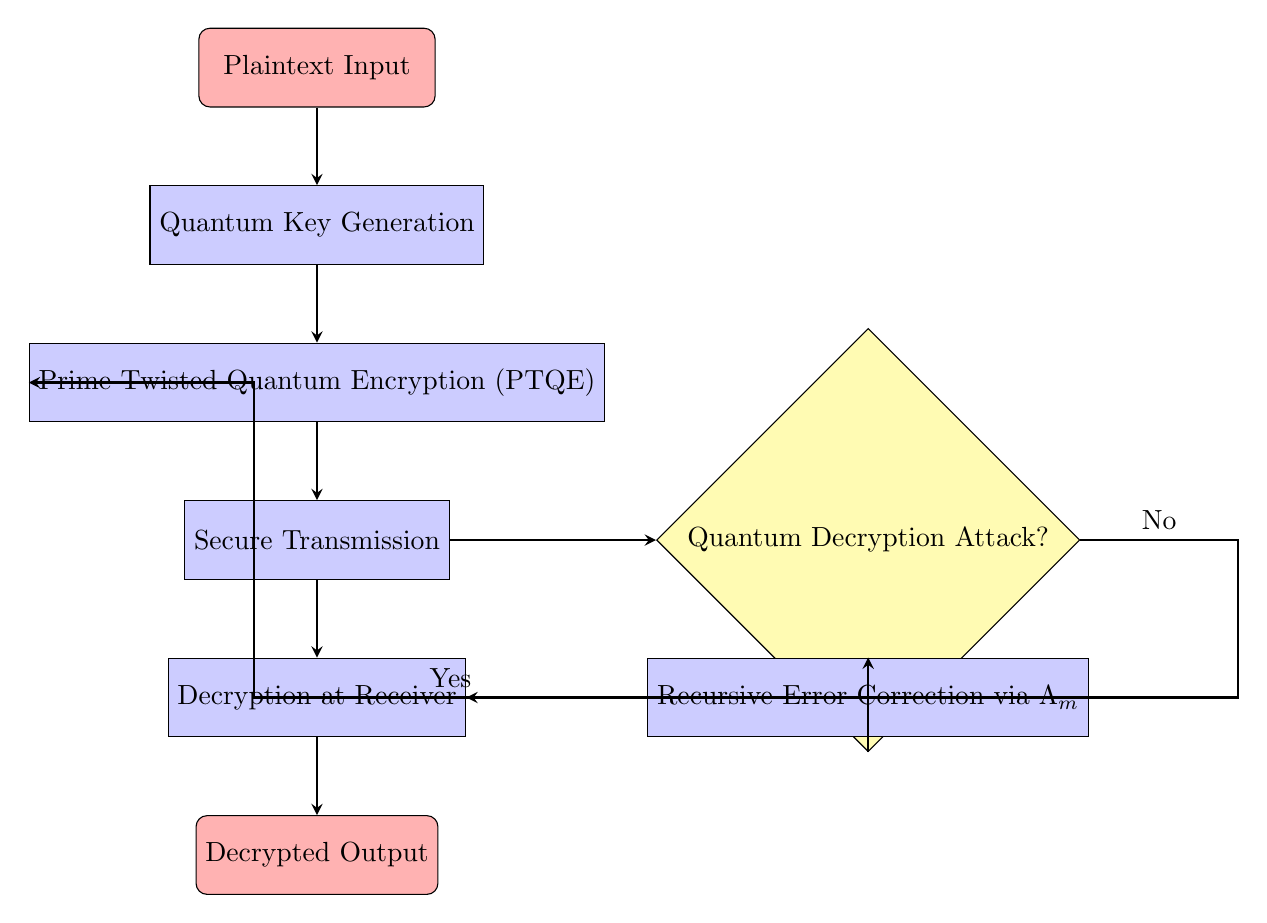
\begin{tikzpicture}[node distance=2cm]

    % Nodes
    \node (input) [startstop] {Plaintext Input};
    \node (quantumkey) [process, below of=input] {Quantum Key Generation};
    \node (encryption) [process, below of=quantumkey] {Prime-Twisted Quantum Encryption (PTQE)};
    \node (securetransmit) [process, below of=encryption] {Secure Transmission};
    \node (attackcheck) [decision, right of=securetransmit, xshift=5cm] {Quantum Decryption Attack?};
    \node (errorcorrection) [process, below of=attackcheck] {Recursive Error Correction via $\Lambda_m$};
    \node (decryption) [process, below of=securetransmit] {Decryption at Receiver};
    \node (output) [startstop, below of=decryption] {Decrypted Output};

    % Arrows
    \draw [arrow] (input) -- (quantumkey);
    \draw [arrow] (quantumkey) -- (encryption);
    \draw [arrow] (encryption) -- (securetransmit);
    \draw [arrow] (securetransmit) -- (decryption);
    \draw [arrow] (decryption) -- (output);
    
    % Attack detection path
    \draw [arrow] (securetransmit.east) -- (attackcheck.west);
    \draw [arrow] (attackcheck.south) -- (errorcorrection.north);
    \draw [arrow] (errorcorrection.west) -- ++(-5cm,0) node[midway,above] {Yes} |- (encryption.west);
    \draw [arrow] (attackcheck.east) -- ++(2cm,0) node[midway,above] {No} |- (decryption.east);

\end{tikzpicture}

\end{document}
